\documentclass[12pt]{article}

\usepackage{graphicx}
\usepackage{float}
\usepackage[latin1]{inputenc}
%% dieses package erlaubt, bei deutscher Tastatur Umlaute, ß direkt einzugeben

\usepackage{siunitx}

\textwidth=170mm
\textheight=240mm
\hoffset= -20mm       % may need change
\voffset= -25mm       % may need change



\begin{document}

%% we do the title page ourselves
\thispagestyle{empty}     % only for frontpage
\null
\vspace{40mm}
\begin{center}
{%%%%%%%%%%%%%%%%%%%%%%%%%% Titel
\Large  CCD photometry
\footnote{\noindent Experiment F30, performed on 3/8/18, Tutor Sarah, long evaluation}}[15mm]
%%%%%%%%%%%%%%%%%%%%%%%%%%% Authors
Lasse Gresista and Benjamin Haake

\vspace{25mm}

\parbox{0.9\textwidth}{   %% etwas schmaler als normaler Satz
Abstract:    
\small The abstract should preferentially be in English. Here we explain in a
few lines (i) what was done, and (ii) what the results were.
}
\end{center}

\vfill
Attested as special evaluation: Date, Signature:
\vspace{20mm}

%% Rueckseite des Titelblatts leer. Bei einseitigem Druck entfernen
\newpage  
\null\thispagestyle{empty} 
   
%\newpage     % Inhaltsverzeichnis, koennte man bei langer Version machen
%\tableofcontents 

\newpage

\pagenumbering{arabic} %% start page 1 
\section{Introduction}
	In this experiment we wanted to familiarize ourselves with the way a CCD detector works and construct a Colour-Magnitude-Diagram of a starcluster. %Since we could not make our own measurements, we analyzed the data by the Hubble space telescope of BS90.

CCD: how does it work, advantages, why cool it, overscan, bias, flat-field(?), noise formulas

Evaluation: magnitudes, HRD and CMD
\begin{equation}
	a\cdot T^{3/2} \exp(-E/(2k_BT))
	\label{BG}
\end{equation}

\section{Magnitude scales}


\section{Setup of the experiment}
	We used the 70cm KING telescope ...
	Filters
	IRAF, DS9, python

\section{Execution}
\subsection{Preparation}
	To get the CCD to working temperature, the dewar the CCD was in was evacuated and filled with liquid nitrogen. The CCD's electronics were then initialized and a test image with closed shutters was taken.\\
	For all measurements the gain factor was 5 and a binning of $2\times2$ pixels was used (A single pixel of the resulting image is therefore 4 pixels of the detector. In all specifications throughout this document in terms of pixels the former are thougth of).
\subsection{Dark current}
	While the CCD was still cooling down, the first set of measurements with exposures of 30s was initialized, controlled by a python script. The temperature was recorded for each image. From these, the dark current can be determined.
\subsection{Flat-field}
	The lid was removed and the telescope was pointed at the blanket on the inside of the dome. It was illuminated by a lightbulb, while all other lightsources in the room were turned off, and a test image was taken. This was done for the filters I,V and R. The exposure time was determined from the test images in such a way to avoid saturation while still having a good signal to noise ratio, i.e. a high intensity (the intensity is not constant for a fixed integration time, since the spectrum of the light source and the quantum efficiency of the detector are not uniform and therefore change when switching filters). Since it was known that the detector would saturate for about $60000$ADU, an illumination time was chosen such that the counts were between $30000$ADU and $40000$ADU. Five images were taken for each filter with exposure times of 4s (I),6s (R) and 30s (V). A master flat-field can be constructed from these images.
\subsection{Linearity}
	To verify the linearity of the detector and determine its dynamical range, 15 images with varying exposure times were taken. The setup was the same as for the flat-field, using only the V-filter. After each image, the exposure time was increased by 4s, starting at 2s.
\subsection{Sensitivity of the detector and noise properties}
	To measure the noise in the detector a similar setup to the linearity measurement is needed. Exposures are taken of the uniformly illuminated surface (blanket) with different exposure times. This time all exposures are taken in the I-Filter. To eliminate the PRNU-Noise, two measurements for each exposure time are taken to later be subtracted from each other. This is done for exposure times from 0.40s to 8.80s in steps of 0.40s. The maximum exposure time is choosen so that the last exposures will be saturated. 
\subsection{Color Magnitude Diagram}
	Since the weather conditions on the days of our lab course where not suited to make our own observation with the telescope at the MPIA, in this section data of the Hubble Space Telescope of the globular cluster BS90 was used. The pictures where taken in the V- and I-filters. A color magnitude diagram will be produced to make an estimation of the age, distance and metallicity of the cluster.

\section{Analysis}
\subsection{Dark current}
	Using IRAF, the temperature was extracted from each image, as well as the biases and their standard deviations from the overscan region. In order to obtain the bias, the median and standard deviation of the region [1025:150,11:1010] were determined. In this exeriment, the median was always used instead of e.g. the mean, since the median is less sensitive to extreme outliers like dead pixels (when taking the median of a single image) or cosmics (when composing a median image from multiple exposures). The measurements were then corrected for their respective bias by subtracting it from each pixel. From these corrected images, the dark current was determined by taking the median value (excluding the overscan region).\\
	These values were then divided by $T^{3/2}$ and logarithmicly plotted against the inverse temperature $\frac{1}{T}$ (see figure \ref{bandgap}). The dependence from equation \ref{BG} was then fitted, the resulting band gap is $E_g = (1,3034 \pm 0,0061)\si{eV}$.
The band gap of Silicon is $E_{g,Si} = 1,15 \si{eV}$ (according to \cite{sc}), which is significantly lower.
\begin{figure}[H]
  \centering
  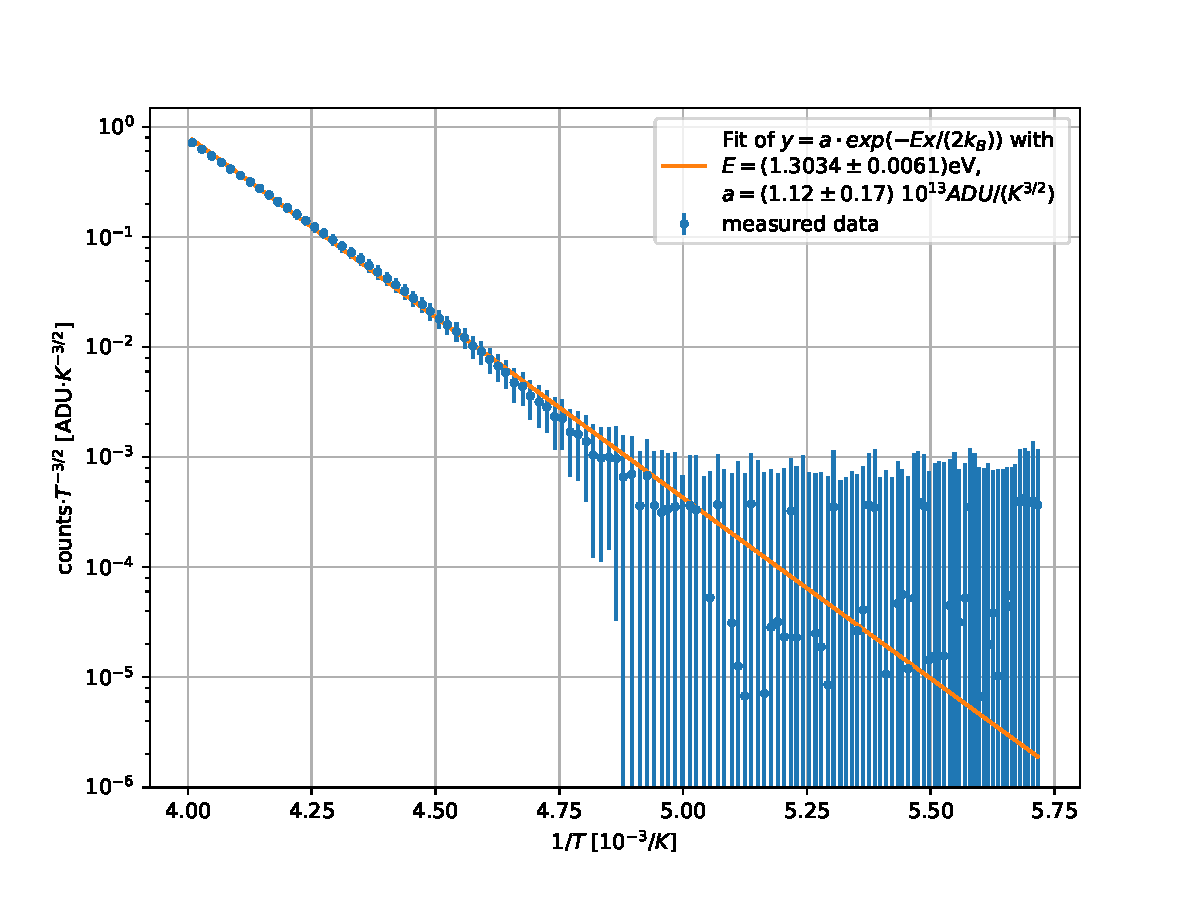
\includegraphics[width=0.8\textwidth]{figures/bandgap.pdf}

%% \label{eichnung} bewirkt, dass \ref{eichung} die Bildnummer gibt.
  \caption{Determination of the bandgap $E_g$ of the detector}
  \label{bandgap}          
\end{figure}
The deviation might be a result of impurities or doping of the semiconductor. Another source of noise that might lead to this deviation is cosmics. It should also be noted that the errors become quite large for low temperatures and a systematic error seems to occur, leading to some values forming a constant line.\\
Comparing the biases of the first ($b=1317,0\pm 2,0$) and last measurement ($b=1345,0\pm 1,7$), we conclude that the bias depends on temperature since it changes significantly over the course of the measurements. This hypothesis is supported by the fact that the bias increases nearly monotonously when the temperature decreases. This dependence on temperature necessitates taking the bias for each image individually.
\subsection{Flat-field}
	As before, the (median) bias was determined from the overscan region of each image and the bias was subtracted from it. As we made 5 images at a fixed exposure time for 3 filters, we took the median (pixel by pixel) of the bias-corrected images with IRAF in order to get a single master flat-field (for each filter). These were normalized by dividing by their median. A histogram of the flat-fields values was created using IRAF and python (see figures \ref{Hist_I} , \ref{Hist_V} and \ref{Hist_R}). 
%\begin{figure}[H]
%	\centering
%	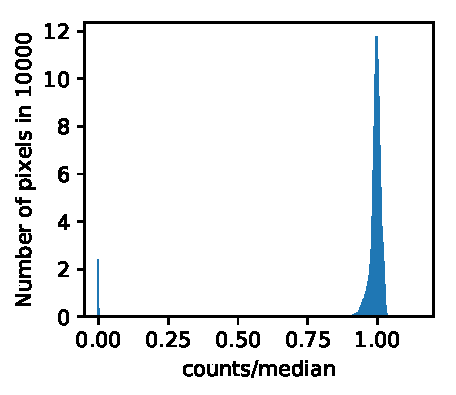
\includegraphics[scale=1]{figures/Hist_I.pdf}
%	\caption{Histogram of the counts by pixel in the I filter, relative to the median}
%	\label{Hist_I}
%\end{figure}
%\begin{figure}[H]
%	\centering
%	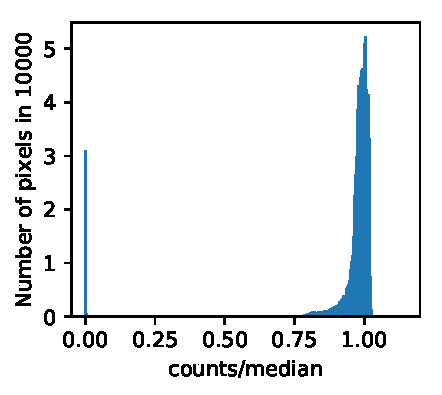
\includegraphics[scale=1]{figures/Hist_V.pdf}
%	\caption{Histogram of the counts by pixel in the V filter, relative to the median}
%	\label{Hist_V}
%\end{figure}
%\begin{figure}[H]
%	\centering
%	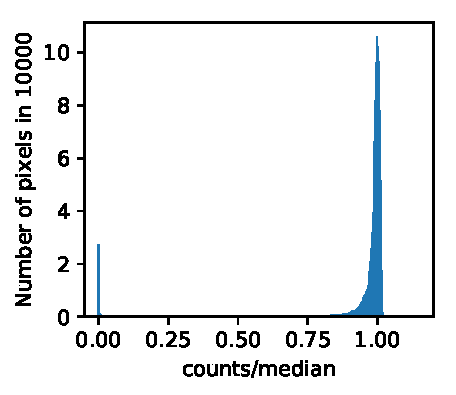
\includegraphics[scale=1]{figures/Hist_R.pdf}
%	\caption{Histogram of the counts by pixel in the R filter, relative to the median}
%	\label{Hist_R}
%\end{figure}
\begin{figure}[H]
\begin{minipage}[t]{0.32\textwidth}
	\centering
	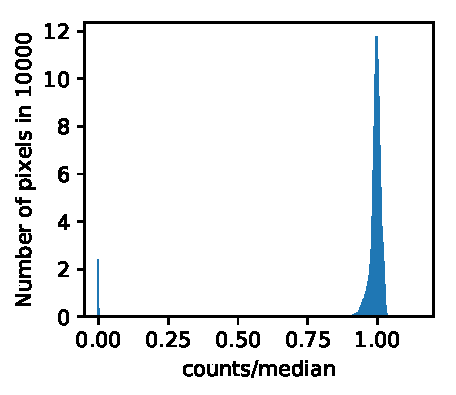
\includegraphics[width=\textwidth]{figures/Hist_I.pdf}
	\caption{I-filter}
	\label{Hist_I}
\end{minipage}
\begin{minipage}[t]{0.32\textwidth}
	\centering
	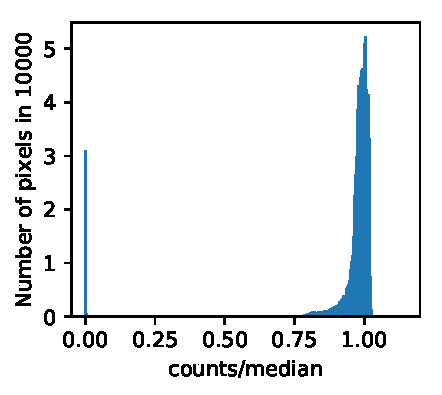
\includegraphics[width=\textwidth]{figures/Hist_V.pdf}
	\caption{V-filter}
	\label{Hist_V}
\end{minipage}
\begin{minipage}[t]{0.32\textwidth}
	\centering
	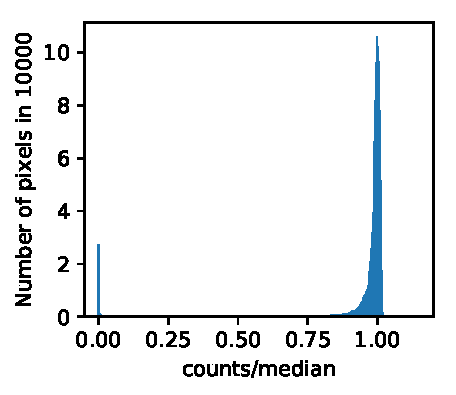
\includegraphics[width=\textwidth]{figures/Hist_R.pdf}
	\caption{R-filter}
	\label{Hist_R}
	\end{minipage}
\end{figure}
	Most values are around 1, which is to be expected. The dark rings that can be seen in figure \ref{BA} create the slight asymmetry of the peak, the overscan region of around 25000 pixels leads to a thin peak at 0. The latter is slightly enhanced by the dark corners of the images, which might come from the detector blocking parts of the light and, of course, dead pixels.\\
	In principle, the master flat-field does not need to be normalized, since a constant factor (the median of the master flat field) would simply shift the zero point in the magnitude scale, which is eliminated by comparison with standard stars anyway.\\
%
	To see the effect of dividing by the master flat-field explicitly, this was done with the second image taken with the I-filter (see figure \ref{BA}).
\begin{figure}[H]
	\centering
	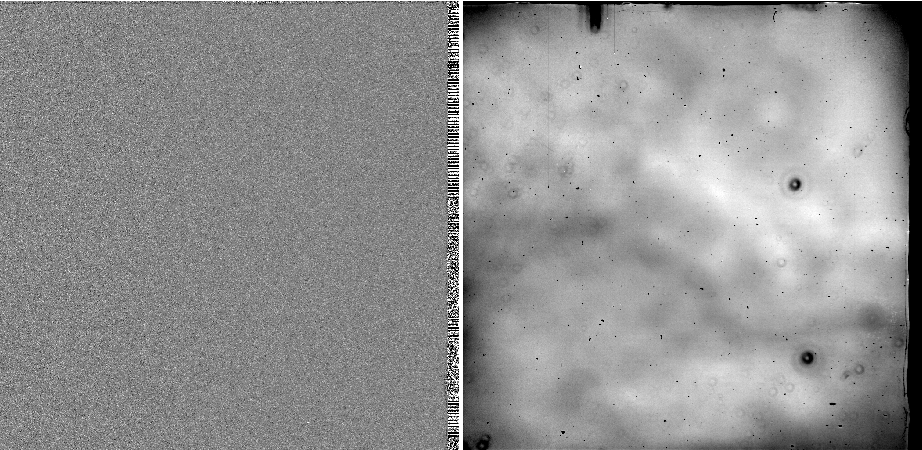
\includegraphics[width=0.8\textwidth]{figures/beforeafter.png}
	\caption{Comparison between the flat-field image (right) and the same image divided by the normalized master flat-field (left).}
	\label{BA}
\end{figure}
This has to be done in principle for every scientific image, since it nullifies the differences between individual pixels due to differing quantum efficiency and differences in illumination (dark corners from the detector and small dark rings). The rings are probably the result of dust particles on the filter. Since the telescope is built to focus on very distant objects (i.e. stars), the blanket used to obtain the flat-field is out of focus and the nails and the variations in illumination due to the curvature of the surface are blurred so much as to become irrelevant.
\subsection{Linearity}
	First, all images were corrected by subtracting their bias and dividing by the master flat-field (of the respective filter). Determining the median, standard deviation and exposure time with IRAF, the median was plotted against the exposure time. This was done in the V- and I-filter (the latter ones are the first set of images of the section "sensitivity").
	
\begin{figure}[H]
	\centering
	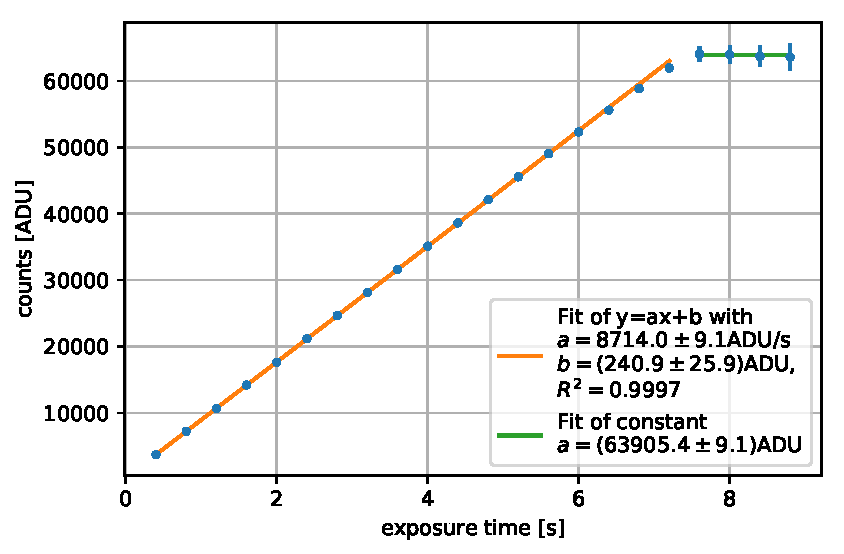
\includegraphics[width=0.6\textwidth]{figures/linearity_I.pdf}
	\caption{Verifying the linearity of the detector (I-filter). This measurement shows that the detector signal is proportional to the integration time with less $0.3\%$ than deviation.}
	\label{linearity_I}
\end{figure}
\begin{figure}[H]
	\centering
	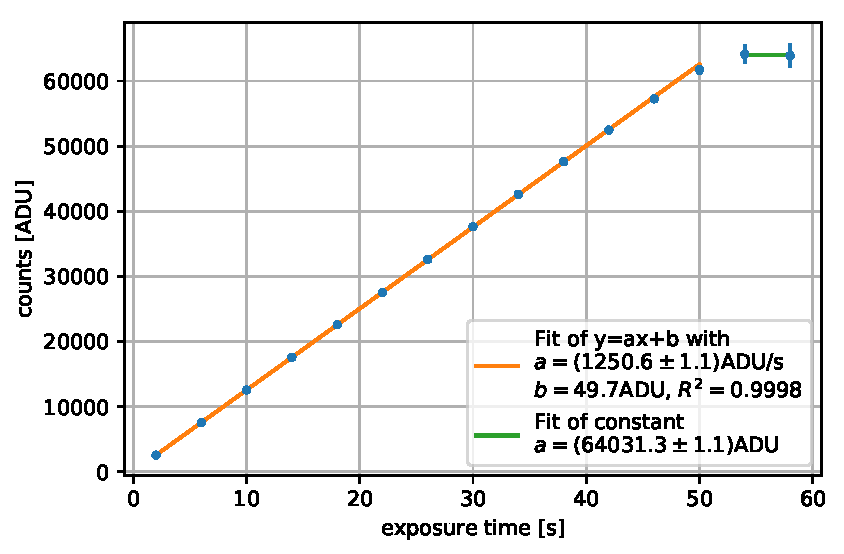
\includegraphics[width=0.6\textwidth]{figures/linearity_V.pdf}
	\caption{Verifying the linearity of the detector (V-filter). This measurement shows that the detector signal is proportional to the integration time with less $0.2\%$ than deviation.}
	\label{linearity_V}
\end{figure}
	From these measurements one can conclude, that the linearity is really good ($R^2\geq 1-3\cdot 10^{-4}$ for both filters) and the detector is linear nearly over its entire dynamical range (counts up to $64000$ADU for a gain factor of 5).
\subsection{Sensitivity of the detector and noise properties}
Initially two images of equal exposure time had to be choosen so that the average signal did not exceed 30000 counts (in ADU). We choose the images with an exposure time of 1.60s. To determine the read-out noise in the two images, the standard deviation of the pixels in the overscan region is calculated using the IRAF routine imstat. For this, the region with x-coordinates reaching from 1025 to 1050 and y-coordinates reaching from 11 to 1010 was selected. Since in the overscan region no physical signal and therefore no physical noise is present, the only noise left is the read-out noise, which means the the calculated standard deviation corresponds directly to the read-out noise. This yielded a read-out noise of $\sigma_{R,d,1}=1.846ADU$ for the first and $\sigma_{R,d,2}=1.845ADU$ for the second image.

Next a region that was as uniformly illuminated as possible had to be choosen, because in the next steps no flat field correction was done. In our case this was the region with x-coordinates 181 to 407 and y-coordinates 195 to 436. From this region we determined the median signal $N_{e,d}$ and the total noise $\sigma_{t,d}$ again using the IRAF routine imstat. This yielded $N_{e,d,1}=14540ADU$, $N_{e,d,2}=15448ADU$, $\sigma_{t,d,1}=206ADU$ and $\sigma_{t,d,2}=205.9ADU$. To eliminate the PRNU-noise one image was subtracted from the other for each pair of images using the IRAF routine imarith. Then the remaining noise $\sigma_{diff,d}$ was calculated in the same region as above for each image pair. For the images with exposure time 1.60s this yielded $\sigma_{diff,d}=53.86ADU$. Additionally the median signal $N_{e,d}$ in the same region was determined for every image and averaged for each image pair. These values will be used plot the variance against the median signal to calculate the gain $\kappa$ of the analog digital converter.

To compare the different relevant noise sources, the photon noise $\sigma_{e,d}$ and the PRNU noise $\sigma_{PRNU,d}$ still had to be calculated. The photon noise was calculated by rearanging equation (*) to 
\begin{equation}
 \sigma_{e,d}=\sqrt{\frac{\sigma_{diff,d}^2-\sigma_{R,d}^2}{2}}
\end{equation}
and the PRNU noise by rearanging equation (*) to
\begin{equation}
 \sigma_{PRNU,d}=\sqrt{\sigma_{tot,d}^2-\sigma_{e,d}^2-\sigma_{R,d}^2}
\end{equation}
Doing this for the first image of the pair with exposure time of 1.60s yields $\sigma_{R,d}=1.846ADU$, $\sigma_{e,d}=38.04ADU$ and $\sigma_{PRNU,d}=202.45ADU$. The PRNU-noise clearly dominates at this signal level. This is expected, since equation (*) with a PRNU factor $f_{PRNU}$ in the order of 0.01 shows that photon noise and PRNU noise are the same at a signal level of about 10 000 electrons.  The signal in ADU was $N_{e,d,1}=14540ADU$ and it will later be shown that the gain (electrons/ADU) was around $\kappa\approx10$, so the signal level was clearly above that regime. Since the PRNU noise grows linearly and the photon noise grows with $\sqrt{N_e}$ the PRNU noise will dominate at these signal levels. In fact the lowest signal level in this measurment (the first exposure) was $5016ADU$ so PRNU is the dominant source of noise for all off our measurements in this section. This is however not a big problem in physical measurements, since the PRNU noise is a result of the different quantum efficiency in the pixels of the CCD, which will be removed by dividing the images by a flat field. This means in physical observations the relevant sources of noise are the read-out noise and the photon noise. The read-out noise is very small resulting in a very big dynamical range of the CCD allowing the observation of very faint objects with reasonable signal to noise ratio. 

To see the correlation between the noise (or variance) of the signal and the signal level itself, we plottet the obtained total variance of the difference image $\sigma_{diff,d}^2$ against the median signal level as seen in figure \ref{fig: sensitivity}.
\begin{figure}[h]
\centering
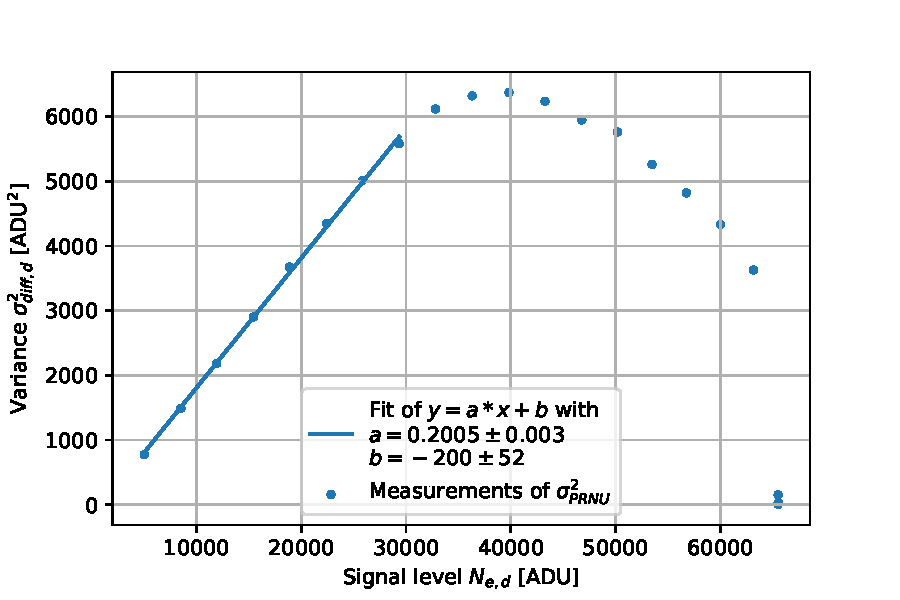
\includegraphics[width=1\textwidth]{figures/sensitivity_plot.pdf} 
\caption{Variance of the difference image against signal level}
\label{fig: sensitivity}
\end{figure}

This plot shows that with at low exposure times and hence low signal levels you  have a linear relationship, as equation (*) suggest. But with increasing signal levels saturated pixels begin to appear. Looking at the maximum count value in the images (Fits Header, Keyword 'DATAMAXI') it was obtained that this starts to happen after the 5th image with an exposure time of 2 seconds. Because saturated pixels have a fixed value, no noise but the readout noise will be left in these pixels. As the amount of saturated pixels grows with the signal level, the variance deviates from a linear relationship and gets even gets smaller after a signal level of about 40 000ADU is reached. This also explains the sudden drop in the variance in the last two picutres, as they were nearly completely saturated, leaving only the variance caused by the read-out noise. To calculate the gain $\kappa$ a linear fit was done to the first 8 measurements. Equation (*) shows that one can extract the gain $\kappa$ and its error from the slope a of the fit with the following equation: 
\begin{equation}
\kappa=\frac{2}{a} 
\end{equation}
\begin{equation}
\Delta\kappa=2\cdot \sqrt{\frac{\Delta a}{a^2}}
\end{equation}
This yields $\kappa=9.97\pm0.14$. One can also obtain the gain using equation (*) from just one image. We choose the first image of the 8th image pair with an exposure time of 3.20s and an average count of about 30 000ADU. The photon noise was calculated using equation (*) which yielded $\sigma_{e,d}=41.16ADU$. Assuming that the quantum efficiency is 1 this yields a gain of $\kappa_8=19.37$. This is a significant deviation to the  first value. In the first method used, it was assumed that the read-out noise is independent of intensity, but by looking at the standard deviation of the pixels in the overscan region, one can see that the read-out noise grows with intensity. This increases the slope of the fit and in turn lowers the value for $\kappa$. The intercept b of the fit with the y-axis corresponds to $2\sigma_{R,d}$, so a negative value does not make physical sense. This might also be explained by the non constant read-out noise, and again suggests an underestimation of the gain $\kappa$. Since the read-out noise itself is still relatively small (under 50 ADU) for these images, the resulting error will also only be of about that order.  In the second method, the read-out noise was determined from the standard deviation of the entire overscan region. Since the signal level in the overscan region showed significant differences in the vertical direction, mainly two jumps of about 50 ADU and a relatively constant value between those jumps, the read-out noise was probably overestimated causing a much larger gain. As mentioned above, saturated pixels appeared in the image used reducing $\sigma_{diff,d}$ and in turn also increasing the value of $\kappa$.  So the first method, which took several images into account, is probably a better estimate for the real value of the gain $\kappa$.

The small deviation of the variance $\sigma_{diff,d}^2$ from a linear relationship ($R^2=0.9988$) shows that the analog digital converter seems to have a very constant gain. This is supported by the linearity segment, where a non constant gain would have also resulted in a bigger deviation from the linear relationship. 

\subsection{Color Magnitude Diagram}
\subsubsection{Zero point calibration}
To convert the instrumental magnitudes of the hubble images into  the apparent magnitude scale, we had to find the zero point magnitude. To do this the catalog "Cool evolved stars in SAGE-SMC and SAGE-LMC (Boyer+, 2011)" was used. The magnitudes of the stars in the catalog as well as the counts in the hubble images are needed to calculate the zeropoint. We selected 10 stars in the catalog, trying to only select isolated stars with as few nearby light sources as possible. This wasn't possible for all selected stars and the determined magnitudes probably also contain small amounts of counts from nearby light sources. The counts in the hubble images were determined by selecting a circular region around the star and obtaining the total count in these regions using the program DS09. The zero point was then calculated for each star in the I- and V-filter using the following equation:
\begin{equation}
zeropoint=m_{CATALOG}+2.5log_{10}(counts)
\end{equation}
To get the final zero point we took the median of all stars. The results were $zeropoint_I=25.09$ and $zeropoint_V=25.34$ 

\subsubsection{Creating the CMD}
To do PSF photometry the program STARFINDER was used. For this we had to select 10-30 isolated stars from which the program calculates a median PSF. It does this by subtracting a background, normalizing the peak intensity and averaging the PSFs of all selected sources. 

To start the process the noise of the image had to be determined also using STARFINDER, so that a treshold relative to that noise can be used for the PSF fitting. The program also lets you plot a histogram of the Gaussian noise (see fig(*)). 


The PSF was then produced with a size of 50 pixels and a diameter of 9 pixels. It can be seen in figure \ref{fig:PSF_V} and \ref{fig:PSF_I}. 
\begin{figure}[h]
  \centering
% hier schon der komplixiert Fall, dass 2 Bilder nebeneinander gesetzt werden
  \parbox{80mm}{
    \centering
    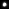
\includegraphics[width=0.3\textwidth]{figures/PSF_V_n.png}
    \caption{PSF in the V filter}
    \label{fig:PSF_V}
  }
  \parbox{80mm}{
    \centering
    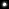
\includegraphics[width=0.3\textwidth]{figures/PSF_I_n.png}
    \caption{PSF in the I filter}
    \label{fig:PSF_I}
  }
  
\end{figure}
Now an iterative PSF fitting was done on both images. STARFINDER searches for stars above the detection threshold relative to the noise and fits the PSF to determine the counts. We did two iterations with a threshold setting of 3 in both iterations.  The used correlation threshold was lowered from the standard 0.7 to 0.5, allowing us to find fainter stars but in turn also increasing the chance of different objects being identified as a star.

To plot a CMD only stars could be used that were found in both images, so the fitting results were cross-matched using a python script, which also subtracted the calculated zeropoint magnitude to produce apparent magnitudes in V and I.  With these result, it was now possible to plot the CMD and overplot it with theoretical isochrones. The result can be seen in figure \ref{CMD}. (ANALYSE DES CMD FEHLT HIER NOCH).
\begin{figure}[H]
	\centering
	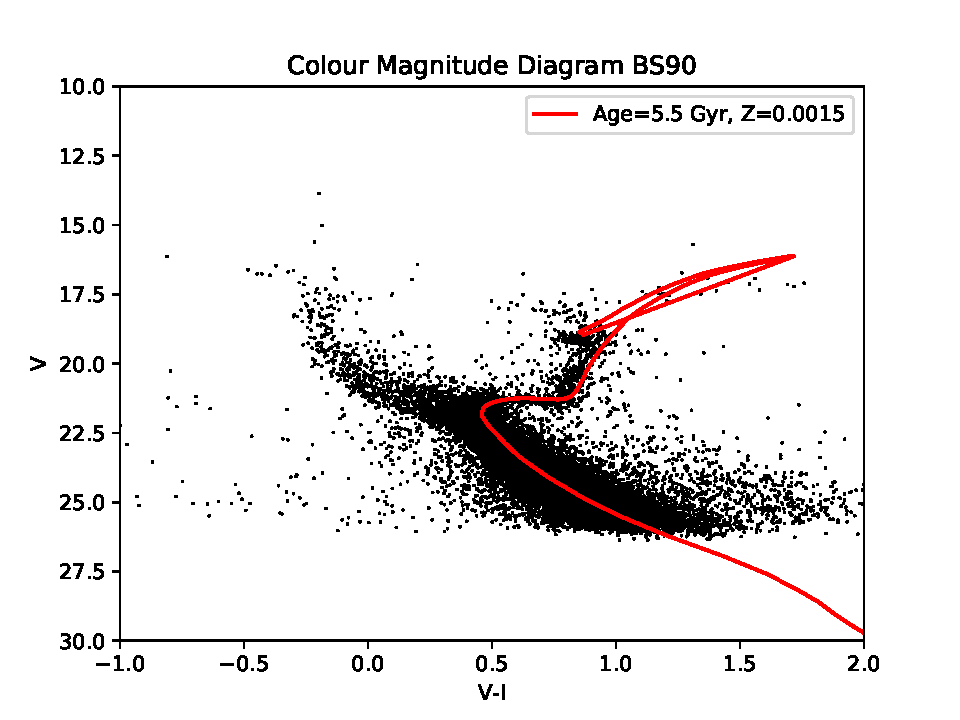
\includegraphics[width=0.7\textwidth]{figures/CMD.pdf}
	\caption{Colour magnitude diagram of BS90 with a model isochrone}
	\label{CMD}
\end{figure}
We adjusted the metallicity Z, the shift in the V-magnitude $\Delta$, which corresponds to the distance modulus, and the age of the isochrone to get the result that best matched our CMD. However this was done by eye, so the results have to be viewed with a big uncertainty. The settings for the isochrone that we though best fitted our CMD were a metallicity of Z=0.0015, a distance modulus of $\Delta=18.5$ magnitudes and an age of 5.5 Gyr. This distance modulus corresponds to a distance of $d=50118$ pc or $d=163594.5$ light-years. These values can be compared to literature values (source*) which are a metallicity of $Z=0.004\pm0.001$, a distance modulus of $\Delta=18.85\pm0.1$ magnitudes and an age of $4.5\pm0.5$ Gyr. Taking into account that we fitted the isochrones by eye, the deviation from our values is relatively small for the distance modulus. Age and metallicity are atleast of the same order of magnitude. Since we don't have a precise measurement of the uncertainty in our measurements, it is hard to judge the validity of our values. 

\section{Discussion}

\newpage
\begin{thebibliography}{00}   % {00}: max 2-stellige Referenznummer

\bibitem{sc} N. Krieger et al., CCD photometry in modern astronomy (2017)

\end{thebibliography}
\end{document}